\chapter{A Common Contract for Stochastic and Legal Operations}\label{ch:jointcontract}

The preceding chapters derived two kinds of preservation. A stochastic instrument can retain the law of the report and successor together. A legal-operation quotient can retain the actions available to a given state and the labels following their execution. Each theorem is useful in isolation, but combining them requires matching the same map, the same state domain, and the same policy interpretation.

Here we prove an explicit finite composition theorem. It is deliberately narrow. The theorem supplies an exact quotient of a \emph{given} model, not a way to infer the model from experience. In particular, it does not derive the legitimacy of an action from mathematical enabled-set data.

\section{The joint data of a decision process}
Let $X$ and $Z$ be finite nonempty sets, $\pi:X\to Z$ a surjection, $A$ a finite action alphabet, and $O$ a finite report alphabet. At each fine state $x\in X$, let $D(x)\subseteq A$ be the set of admissible actions, and let $\ell(x)\in Y$ be a protected label. For every $a\in D(x)$, let
\[
K_{a,o}(x'\mid x)\ge 0,\qquad
\sum_{o\in O}\sum_{x'\in X}K_{a,o}(x'\mid x)=1.
\]
The instrument records one \emph{joint} distribution of next state and report. Correct marginals by themselves are insufficient for sequential correction.

A coarse state $z$ must carry a label $\bar\ell(z)$, an admissible-action set $\bar D(z)$ and one coarse instrument $\bar K_{a,o}(z'\mid z)$ for each $a\in\bar D(z)$. Define $\pi_*\mu$ by summing the mass of a fine distribution over each fibre of $\pi$.

\begin{theorem}[Joint legal and stochastic quotient criterion]\label{r:joint-quotient}
A coarse model exists with
\[
D=\bar D\circ\pi,\qquad \ell=\bar\ell\circ\pi,
\qquad \pi_*K_{a,o}(\cdot\mid x)=\bar K_{a,o}(\cdot\mid\pi x)
\]
for every fine state $x$, every $a\in D(x)$ and every report $o$, if and only if, whenever $\pi x=\pi y$,
\begin{align}
D(x)&=D(y), & \ell(x)&=\ell(y),\label{eq:fibre-legal}\\[-1mm]
\sum_{\pi x'=z'}K_{a,o}(x'\mid x)&=\sum_{\pi x'=z'}K_{a,o}(x'\mid y)
&&\text{for each }a\in D(x),\ o\in O,\ z'\in Z.\label{eq:fibre-joint}
\end{align}
The resulting coarse label, enabled sets and joint instruments are unique. Under any common, potentially randomized policy using only the shared observation history and selecting actions legal in every state consistent with that history, the fine and coarse models induce identical distributions on every finite action/report/label history after matching the initial coarse law $\pi_*p_0$.
\end{theorem}
\begin{proof}
If the quotient data exist, evaluating their three factorization identities at two states in the same fibre proves each condition. For sufficiency, surjectivity gives a representative for every coarse state. Use the common fibre value to define $\bar D(z)$ and $\bar\ell(z)$. For every admitted action and report, set
\[
\bar K_{a,o}(z'\mid z)=\sum_{\pi x'=z'}K_{a,o}(x'\mid x),\qquad \pi x=z.
\]
Equation~\eqref{eq:fibre-joint} makes this independent of the chosen $x$. The entries are nonnegative. Summing across all $z'$ and $o$ partitions the fine next-state space and gives total mass one. Thus the coarse instrument is stochastic on every enabled action. The same fibre argument and surjectivity show uniqueness of all coarse data.

To compare histories, retain the unnormalized fine distribution $p_h$ on the states compatible with a particular joint action/report history $h$. Suppose by induction the corresponding coarse vector is $\bar p_h=\pi_*p_h$. The common policy assigns the same probability $\alpha(a\mid h)$ to its next action in both models. For an admissible $a$ and a subsequent report $o$,
\[
\begin{aligned}
\pi_*p_{hao}
&=\pi_*\bigl(\alpha(a\mid h)K_{a,o}p_h\bigr)\\
&=\alpha(a\mid h)\bar K_{a,o}\pi_*p_h
=\bar p_{hao}.
\end{aligned}
\]
The middle equality holds because the equality of joint fibre sums proves the intertwining identity for each source point mass, and hence for every nonnegative input distribution supported where $a$ is admissible. Linearity handles randomized policies. The initial equality is part of the hypothesis, so induction proves equality on all finite histories, including zero-mass histories. Total mass gives the same history probability; the label factorization gives the same protected label along every retained coarse path. The enabled-set factorization ensures that a common policy does not execute an admitted action in one model while treating it as disabled in the other. No posterior is asserted on a zero-mass report. For positive mass, division by that common mass gives equal aggregated posteriors.
\end{proof}

\paragraph{Scope.} The theorem has finite models, supplied transition/report semantics, a specified common policy and explicit access to its shared history. It does not claim a learner constructs $\pi$, that a latent coordinate is causally adequate, or that the models accurately describe a physical system. The action legality being preserved is the one explicitly encoded by $D$. The theorem does not independently establish normative authority.

\section{Why preserving two marginals is insufficient}
Consider two fine states in the same proposed coarse input fibre. In both, the next coarse state and the next report are individually uniform over $\{0,1\}$. From the first fine state, however, the pairs $(z',o)$ are $(0,0)$ and $(1,1)$ with probability $1/2$ each; from the second they are $(0,1)$ and $(1,0)$ with probability $1/2$ each. The next-state marginal and report marginal agree exactly, yet the report determines opposite next states in the two cases. There is no single coarse \emph{joint} instrument satisfying Equation~\eqref{eq:fibre-joint}.
\begin{figure}[htbp]\centering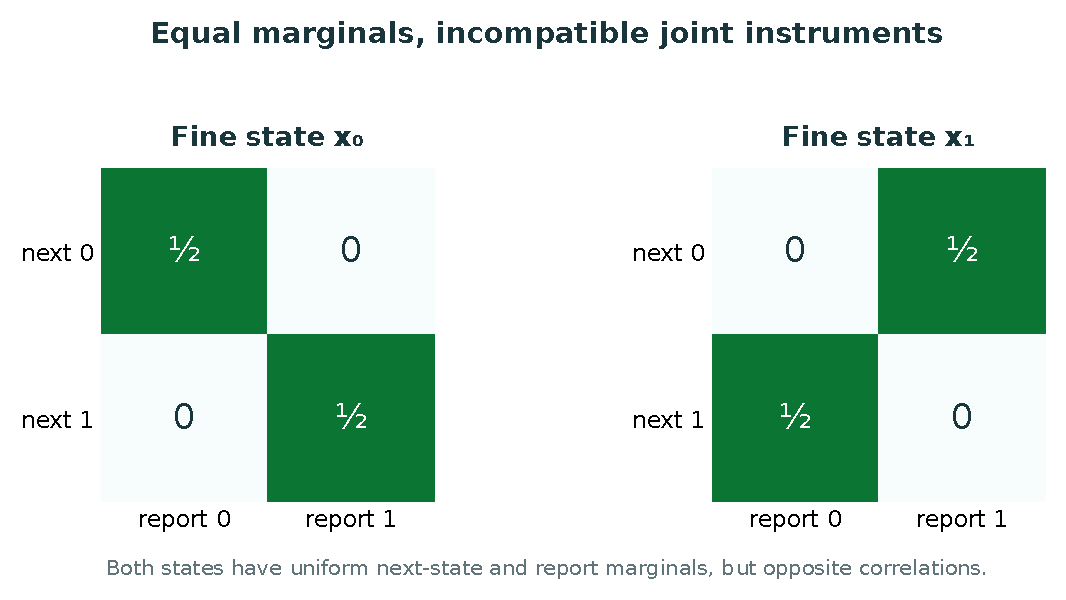
\includegraphics[width=.87\linewidth]{figures/joint_instrument_obstruction.pdf}\caption{Two fine states have identical marginals but incompatible joint report/next-state distributions. The values are exact, not sampled.}\label{fig:joint-obstruction}\end{figure}
This counterexample explains why an abstraction validated only on separate prediction and report tests cannot be promoted to a sequential Bayesian filter without a further condition. One must preserve the association that the next correction uses. The obstruction is structural and persists even in a two-by-two example.

\section{A nuisance-free exact realization}
Return to the eight-world sensor, $x=(b,s,n)\in\{0,1\}^3$, and let the coarse state be $z=(b,s)$. Removing $n$ leaves four coarse states. Offer \emph{hold} and \emph{flip} everywhere, and a \emph{repair} operation only where $b=0$. Let a normal report equal the post-action display $b\oplus s$ with probability $3/4$ and the opposite display with probability $1/4$. Every next state retains the nuisance bit, which the admitted label and action catalogue ignore.

The quotient respects the displayed bit, the enabled-set distinction, and the joint report/next-state law. Given one common policy that uses the report history and only actions legal for all still-possible states, projecting away $n$ commutes with every finite update. The accompanying exact rational verifier enumerates the full fine and coarse history distributions at horizons zero through four, including a report-contingent policy. No observed difference appears because the contracted equations hold identically.

This example does not learn its observation likelihoods. Its probability $3/4$ is an assumption of the model. It also does not permit choosing \emph{repair} from a report alone when the report leaves $b$ ambiguous; that would violate the common-admissibility premise. The distinction is part of the theorem, not an implementation inconvenience.

\section{What composition now permits}
The result has a useful form: local algebraic conditions produce one controlled finite history law, provided observation, legality, and policy semantics remain typed consistently. Three failure modes therefore remain separate. First, a state quotient may destroy the label or enabled-set information. Second, a stochastic quotient may preserve marginals and lose the correlation necessary for correction. Third, a formally valid quotient may be unavailable to a learner because its initializer or model class was never identified from the admitted evidence.

The first two are mathematical obstructions to the proposed representation itself. The third is a question of acquisition. They require different repairs, and this book will not turn them into a single untyped ``representation error.''
